%
%===============>>  Порядин Модуль 8 <<=============
%=
\setmodule{9}

%BEGIN_FOLD % ====>>_____ Занятие 1 _____<<====
\begin{class}[number=1]
	\begin{listofex}
		\item Вычислите:
		\begin{tasks}(2)
			\task \( ( 8 094 \cdot 4 + 24 592 : 8 ) - 24 869\)
			\task \( ( 63 725 + 41 375 - 103 228 ) : 4 \cdot 6 \)
			\task \( 13 257 + 4 326 : 7 \cdot 8 - 7 543 \)
			\task \( ( 60 000 - 32 216 + 54 674 ) : 9 \cdot 3 \)
			\task \( 847 \cdot 8 + ( 42 000 - 39 918) : 6 \)
			\task \( 602 630 - 297 480 : 37 \cdot 69 + 8 653 \)
		\end{tasks}
		\item Караван верблюдов шёл в первый день 8 ч со скоростью 9 км/ч, во второй день – 6 ч со скоростью 8 км/ч, а в третий день – 9 ч со скоростью 7 км/ч. Какое расстояние прошёл караван за 3 дня?
		\item Вертолёт пролетает 840 км за 3 ч, а автомобиль проходит это же расстояние за 7 ч. У кого из них скорость больше и на сколько?
		\item Поезд проходит 320 км за 5 ч. Какое расстояние он пройдёт за 8 ч, двигаясь с этой же скоростью?
		\item Туристы решили пройти за день 30 км. Они уже прошли 3 ч со скоростью 6 км/ч. Какое расстояние им осталось пройти?
		\item За сколько времени они пройдут это расстояние, двигаясь с прежней скоростью?
		\item Ира прошла 15 км за 3 ч, а Петя – 16 км за 4 ч. У кого из ребят скорость больше и на сколько?
		\item Автомобиль за 6 ч проехал 480 км. Какое расстояние мог бы проехать автомобиль за это же время, если бы увеличил скорость на 12 км/ч?
	\end{listofex}
\end{class}
%END_FOLD

%BEGIN_FOLD % ====>>_____ Занятие 2 _____<<====
\begin{class}[number=2]
	\begin{listofex}
		\item .
	\end{listofex}
\end{class}
%END_FOLD

%BEGIN_FOLD % ====>>_ Домашняя работа 1 _<<====
\begin{homework}[number=1]
	\begin{listofex}
		\item .
	\end{listofex}
\end{homework}
%END_FOLD

%BEGIN_FOLD % ====>>_____ Занятие 3 _____<<====
\begin{class}[number=3]
	\begin{listofex}
		\item .
	\end{listofex}
\end{class}
%END_FOLD

%BEGIN_FOLD % ====>>_____ Занятие 4 _____<<====
\begin{class}[number=4]
	\begin{listofex}
		\item .
	\end{listofex}
\end{class}
%END_FOLD

%BEGIN_FOLD % ====>>_ Домашняя работа 2 _<<====
\begin{homework}[number=2]
	\begin{listofex}
		\item .
	\end{listofex}
\end{homework}
%END_FOLD

%BEGIN_FOLD % ====>>_____ Занятие 5 _____<<====
\begin{class}[number=5]
	\begin{listofex}
		\item Занятие 5
	\end{listofex}
\end{class}
%END_FOLD

%BEGIN_FOLD % ====>>_____ Занятие 6 _____<<====
\begin{class}[number=6]
	\begin{listofex}
		\item Занятие 6
	\end{listofex}
\end{class}
%END_FOLD

%BEGIN_FOLD % ====>>_ Домашняя работа 3 _<<====
\begin{homework}[number=3]
	\begin{listofex}
		\item .
	\end{listofex}
\end{homework}
%END_FOLD

%BEGIN_FOLD % ====>>_____ Занятие 7 _____<<====
\begin{class}[number=7]
	\begin{listofex}
		\item Вычислите:
		\begin{tasks}(3)
			\task \( 4 + 5 \cdot (9 + 11) \)
			\task \( 124\cdot4 \)
			\task \( 7 + 3 \cdot (8 + 12) \)
			\task \( 17 + 3 \cdot 3 - 18 \)
			\task \( 53 - 2\cdot 8 + 12 \)
			\task \( 15015 : 5 - 230 \cdot 3 \)
		\end{tasks}
		\item У Тани есть 1500 рублей, и ей нужно купить 2 кг капусты, 1 кг перца, 1 кг моркови и 2 килограмма помидоров. Какое наибольшее число лукошек клубники может купить Таня на оставшиеся деньги?
		\begin{figure}[h]
			\center{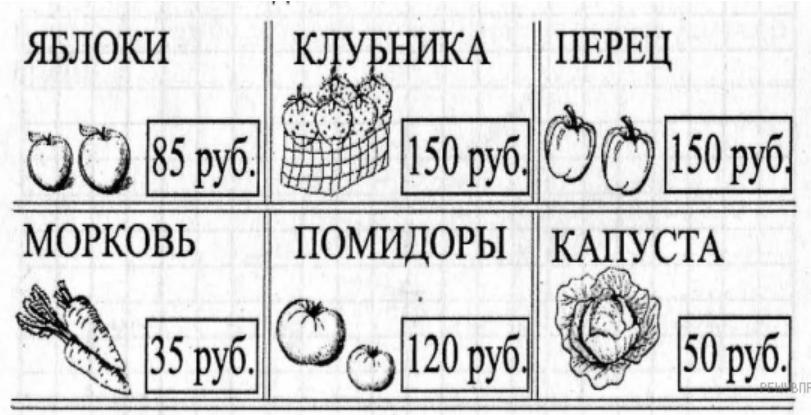
\includegraphics[align=t, width=0.5\linewidth]{../../../../../exercises/lists/pics/poryadin4M8L7}}
		\end{figure}
		
		\item Электричка из Ростова-на-Дону в Краснодар отправилась в 7 часов 40 минут и прибыла в 12 часов 25 минут. Сколько времени занимает дорога из Ростова-на-Дону в Краснодар, если ехать этой электричкой? Ответ вырази в минутах.
		\item Сивый мерин догоняет пони с расстояния 23 520 метров. Через 86 минут между ними оставалось 42 метра. Сколько сивый мерин может проскакать за 2 минуты, если пони скачет 95 м/мин.
		\item Синий трактор едет навстречу телевизору на колёсиках со скоростью в 4 раза быстрее чем у телевизора. Телевизор проезжает в среднем за 42 часа 2436 метров. Встретятся ли они через 79  часов, если расстояние между ними было 22 км?
		
	\end{listofex}
\end{class}
%END_FOLD

%BEGIN_FOLD % ====>>_____ Занятие 8 _____<<====
\begin{class}[number=8]
	\begin{listofex}
		\item \begin{tasks}(2)
			\task \( 12-3+4\cdot(3\cdot5-5) \)
			\task \( 6-2+3\cdot(2+45:8)-7+4\cdot4 \)
			\task \( (25-14)\cdot3-(21-3):9 \)
			\task \( 5\cdot10+4-13\cdot2-1 \)
			\task \( 36:4\cdot5+5-50 \)
			\task \( 23+84:(6\cdot7-12+9\cdot3\cdot2) \)
		\end{tasks}
		\item Паша дразнил гуся на расстоянии 15 м, гусь разозлился и решил пощипать мальчика. Через сколько секунд гусь догонит Пашу, если Паша может пробежать за 44 секунды 262 метра, а гусь за 1 мин 9 с пробегает 621 м?
		\item Вова и Неля играют в догонялки. Неля бегает со скоростью 
		4 м/с, а Вова может пробежать за 4 секунды 20 метров. Вова убегает от Нели - какое расстояние будет между ними 
		через 10 секунд?
		\item От двух пристаней навстречу друг другу одновременно вышли теплоход и катер. Теплоход шёл со скоростью 33 км/час, а катер --- 25 км/час. Через 3 часа они встретились. Чему равно расстояние между пристанями?
		\item Осьминог и каракатица испугались друг дружку и поплыли в разные стороны. Через 37 секунд между ними оказалось 2 516 дециметров. Сколько каракатица проплывает за 201 секунду, если осьминог плавает на 14 дм/с быстрее.
		\item  Из двух городов, расстояние между которыми 840 км, вышли одновременно навстречу друг другу 2 поезда. Скорость первого поезда --- 100 км/час, второго --- на 10 км/час больше. Через сколько часов поезда встретятся?
	\end{listofex}
\end{class}
%END_FOLD

%BEGIN_FOLD % ====>>_____ Домашняя работа 4 _____<<====
\begin{homework}[number=4]
	\begin{listofex}
		\item Вычислите:
		\begin{tasks}(3)
			\task \( 20 + 20 : 5 - 17 \)
			\task \( 24 - 4 \cdot 2 + 15 \)
			\task \( 18 + 4 \cdot 3 - 11 \)
			\task \( 49 - 8 \cdot 3 - 16 \)
			\task \( 6 + 27 : 3 + 19 \)
			\task \( 12 + 24 : 4 + 23 \)
		\end{tasks}
		\item Масса восьми одинаковых ящиков с черносливом равна 100 кг. Масса пустого ящика равна 500 грамм. Чему равна масса чернослива в одном ящике?
		\item Сивый мерин догоняет пони с расстояния 23 520 метров. Через 86 минут между ними оставалось 42 метра. Найдите сколько сивый мерин может проскакать за 2 минуты, если пони скачет 
		95 м/мин.
		\item Синий трактор едет навстречу телевизору на колёсиках со скоростью в 4 раза быстрее чем у телевизора. Телевизор проезжает в среднем за 42 часа 2436 метров. Встретятся ли они через 79  часов, если расстояние между ними было 22 км?
		\item Осьминог и каракатица испугались друг дружку и поплыли в разные стороны. Через 37 секунд между ними оказалось 2 516 дециметров. Найдите сколько каракатица проплывает за 201 секунду, если осьминог плавает на 14 дм/с быстрее.
	\end{listofex}
\end{homework}
%END_FOLD